\section{Design overview}
\label{sec:matrix}


The objective of Matrix is to enable any-to-any routing in an
underlying data collection protocol for 6LoWPAN, such as CTP and
RPL, while preserving memory and message efficiency, as well as
adaptability to networks topology dynamics\footnote{Note that Matrix
is not designed to address scenarios with node mobility, but only to
work with network topology dynamics caused by changes in link
quality, as well as node and link failures.}. Matrix is a network
layer protocol that works together with a routing protocol.
Figure~\ref{fig:architecture} illustrates the protocol's
architecture, which is divided into: \textit{routing engine} and
\textit{forwarding engine}. The routing engine is responsible for
the address space partitioning and distribution, as well as routing
table maintenance. The forwarding engine is responsible for
application packet forwarding.

\begin{figure}[!ht]
    \centering
    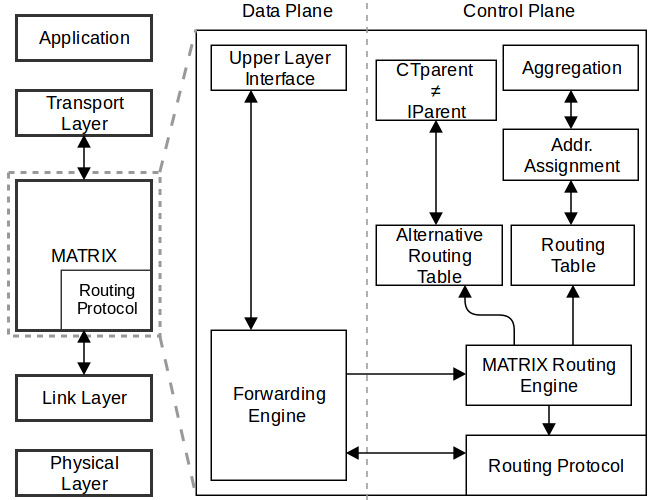
\includegraphics[width=1\columnwidth]{./Images/Architecture.png}
\caption{Matrix protocol's architecture.}
    \label{fig:architecture}
\end{figure}

Matrix is comprised of the following execution phases:
%\begin{enumerate}
 % \item
 
\noindent \textbf{1. Collection tree initialization}: the
  collection tree (Ctree) is built by the underlying collection protocol; each
  node achieves a stable knowledge about who its parent is; adaptive beaconing
  based on Trickle algorithm \cite{Levis:2004} is used to define stability;
  
%  \item
\noindent  \textbf{2. Descendants convergecast,
  IPv6 tree broadcast}: once the collection tree
  is stable, the address hierarchy tree (IPtree) is built using MHCL
  \cite{mhcl}; this phase also uses adaptive beaconing to handle network
  dynamics; by the end of this phase, each node has received an IPv6 address
  range from its parent and each non-leaf node has partitioned its own address 
	space among its children; the resulting address
  hierarchy is stored in the distributed IPtree, which initially has the same
  topology as Ctree, but in reverse, top-down, direction.
  
%  \item
\noindent  \textbf{3. Standard routing}: bottom-up routing is done
  using the collection tree, Ctree, and top-down routing is done using the
  address hierarchy represented by the IPtree; any-to-any routing is performed by combining
  bottom-up forwarding, until the least common ancestor of sender and
  receiver, and then top-down forwarding until the destination.
  
%  \item
\noindent  \textbf{4. Alternative top-down routing table upkeep}: whenever a
node changes its parent in the initial collection tree, it starts sending
  beacons to its new parent in Ctree, requesting to upkeep an entry in
  its routing table with its own IPv6 range; such new links in
  Ctree, in reverse direction, comprise the RCtree routing tables for
  alternative (top-down) routing;
  
%  \item 
\noindent  \textbf{5. Alternative top-down routing via local broadcast}:
whenever a node fails to forward a data packet to the next hop/subtree in the IPtree, it
  broadcasts the packet to its one-hop neighborhood; upon receiving a local
  broadcast, all neighbors check if the destination IPv6 belongs to an address
  range in their RCtree table; if positive, the packet is forwarded to the
  correct subtree of IPtree, otherwise, the packet is dropped; we give a
  geometric argument and show through simulations that such events are rare.
%\end{enumerate}

Next we describe the architecture of Matrix in more detail.

\subsection{IPv6 multihop host configuration}

Matrix is built upon the idea of IPv6 hierarchical address
allocation, proposed in \cite{mhcl, 2016techreport}. Once the collection tree is
stable, the address space available to the border router of the
6LoWPAN, for instance the 64 least-significant bits of the IPv6
address (or a compressed 16-bit representation of the latter), is
hierarchically partitioned among nodes in the collection tree. The
(top-down) address distribution is preceded by a (bottom-up)
convergecast phase, in which each node counts the total number of
its descendants, i.e., the size of the subtree rooted at itself, and
propagates it to its (preferred) parent. Each node saves the number
of descendants of each child. 

Once the root has received the
(aggregate) number of descendants of its $k$ children, it partitions
the available address space into $k$ ranges of size proportional to
the size of the subtree rooted at each child, leaving a portion of
the space as reserve for possible late coming connections (see
Figure~\ref{fig:mhcl}). Each node repeats the address space
partitioning procedure upon receiving its own address range from the
parent and sends the proportional address ranges to the respective
children, until all nodes have received an address. If a new node
connects to the tree after the aggregation phase, it receives an
address range from the reserved space of the respective parent node
(the details of the communication routines used in this phase are
described in detail in \cite{2016techreport}).

Since the address allocation is performed in a hierarchical way, each entry in
the routing table aggregates the addresses of all destination nodes
in the subtree rooted at the corresponding child node. 


\begin{figure}[ht]
    \centering
    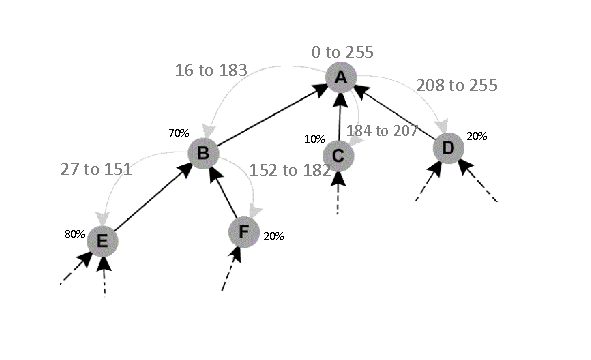
\includegraphics[width=0.9\linewidth]{./Images/mhcl.pdf}
\caption{Example of hierarchical address assignment: (simplified)
scenario with 8-bit available address space at the root and $6.25\%$
of address reserve for delayed connections at each node.}
    \label{fig:mhcl}
\end{figure}

After the address configuration phase, the network initialization is done.
Each node has built the IPtree routing table with the address range of each
child. All table entries are disjoint and sorted in increasing order of
addresses. In this way, message forwarding can be performed in linear time using
one comparison operation per table entry.


\subsection{Control plane: distributed tree structures}

After the network is initialized and all nodes have received an IPv6
address range, three simultaneous distributed trees are maintained
on all nodes in the 6LoWPAN: \textbf{Ctree:} the collection tree, maintained by the underlying
  collection protocol (CTP/RPL).
  %\item 
	\textbf{IPtree:} the IPv6 address tree, built during the network
  initialization phase and kept static afterwards, except when new
  nodes join the network, in which case they receive an IPv6 range from the reserve space of the respective
parent node in the collection tree.
  %\item 
	\textbf{RCtree:} the reverse collection tree, reflecting the
  dynamics of the collection tree in the reverse direction.
%\end{itemize}

Initially, IPtree has the same topology as the reverse-collection tree
$Ctree^{R}$, and RCtree has no links (see Figure \ref{fig:t1} and
\ref{fig:t2}).
$$
IPtree = Ctree^{R} \ \text{and} \ RCtree = \emptyset
$$
%, and any-to-any packet forwarding is performed using Ctree for bottom-up and
% IPtree for top-down data flows, respectively.
Whenever a change occurs in one of the links in Ctree, the new link
is added in the reverse direction into RCtree and maintained as long
as this topology change persists (see Figures \ref{fig:t3} and
\ref{fig:t4}).
$$
RCtree = Ctree^{R} \setminus IPtree
$$

Therefore, RCtree is not really a tree since it contains only the
reversed links present in Ctree but not in IPtree. Nevertheless, its
union with the ``working'' links in IPtree is, in fact, a tree,
which is used in the alternative top-down routing:
$$
RCtree \cup (IPtree \cap Ctree^{R}) \  \text{:alternative routing tree.}
$$

\begin{figure}[!h]
\begin{center}
  \subfigure[]
  {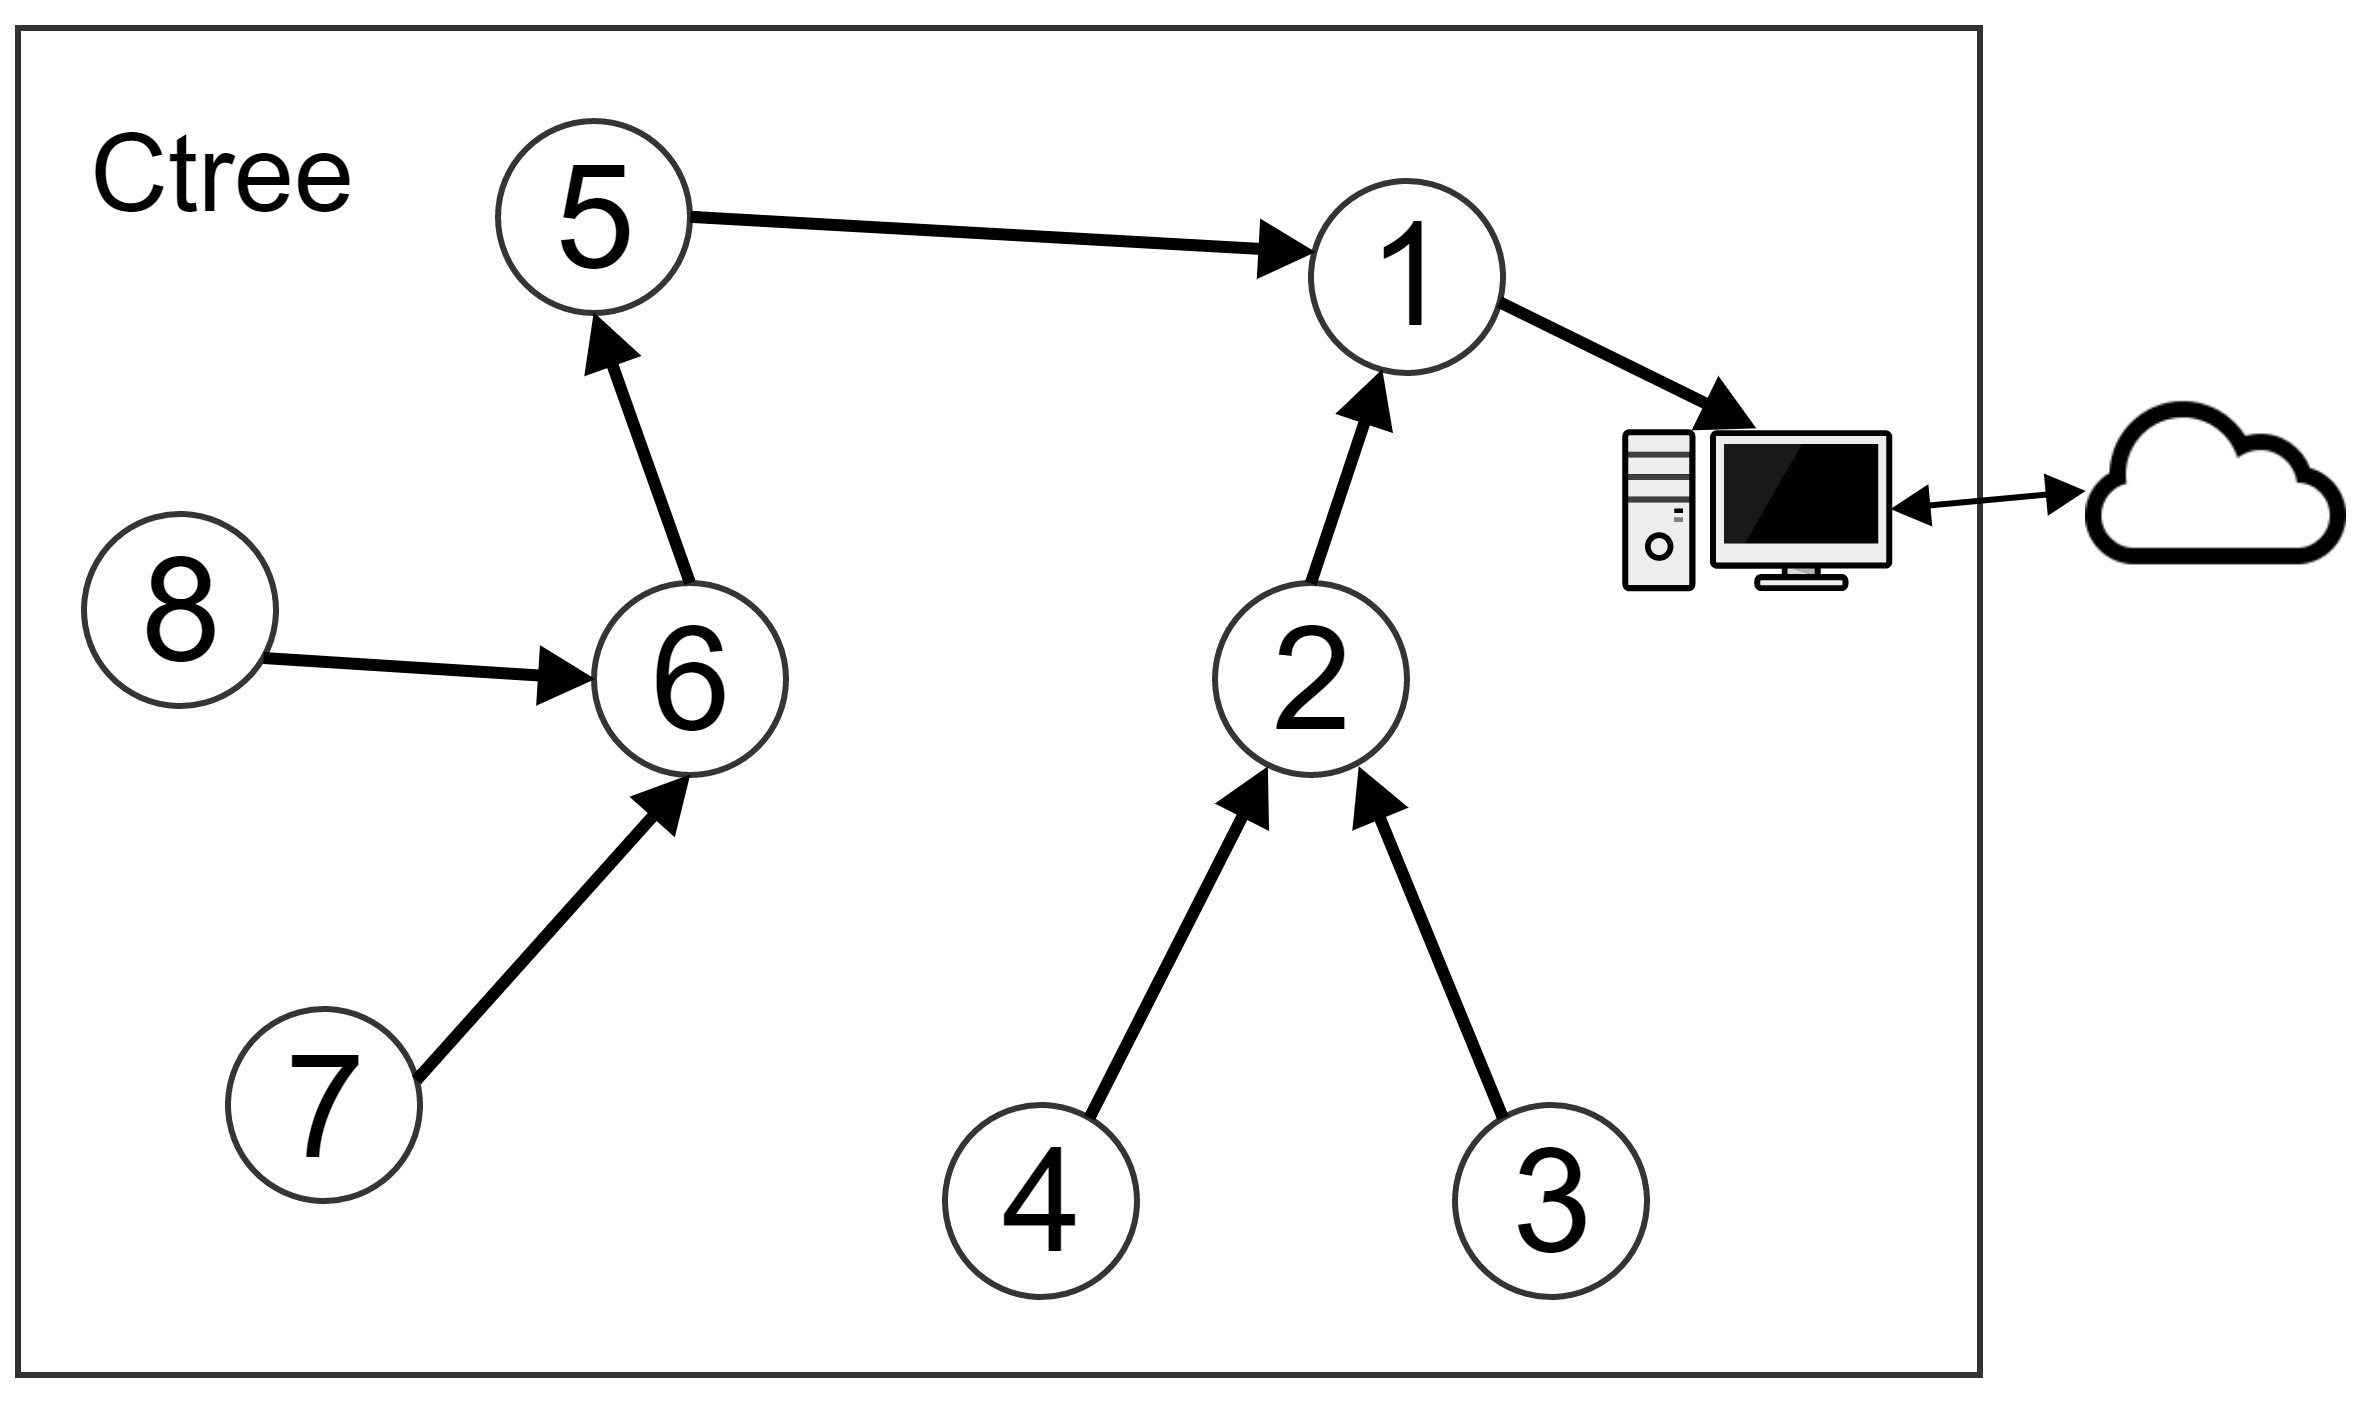
\includegraphics[width=.48\columnwidth]{Images/topologia1.png}
            \label{fig:t1}}
  \subfigure[]
  {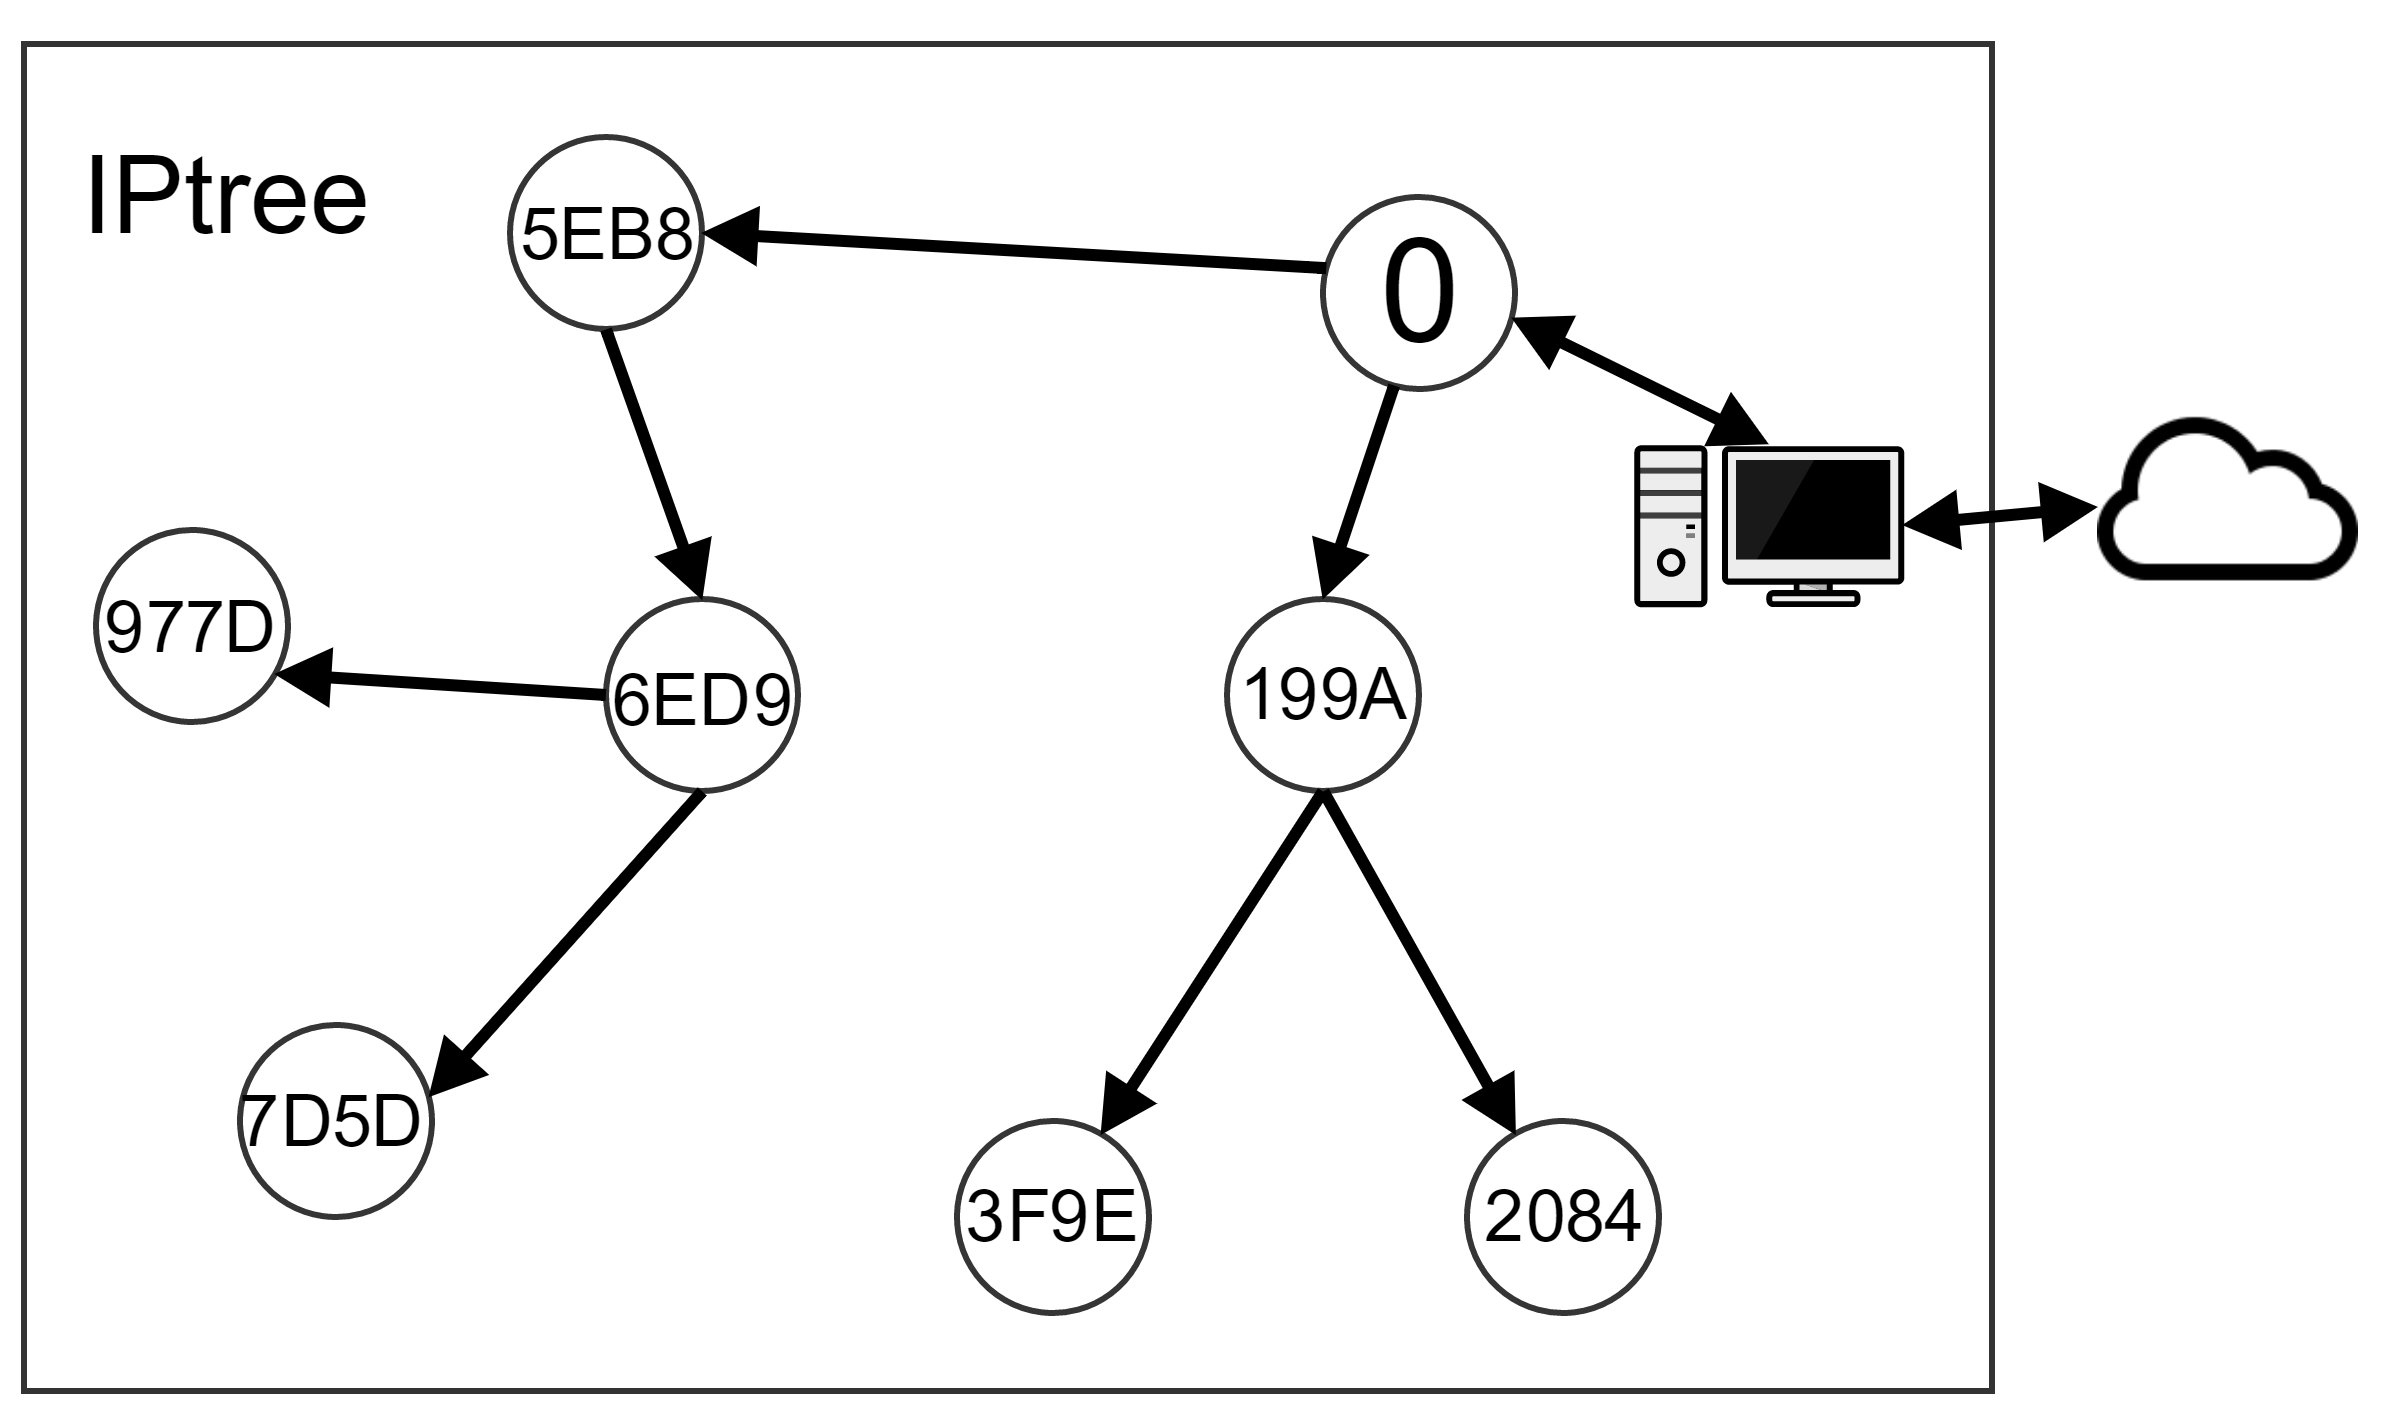
\includegraphics[width=.48\columnwidth]{Images/topologia2.png}
                        \label{fig:t2}}
                            \subfigure[]
  {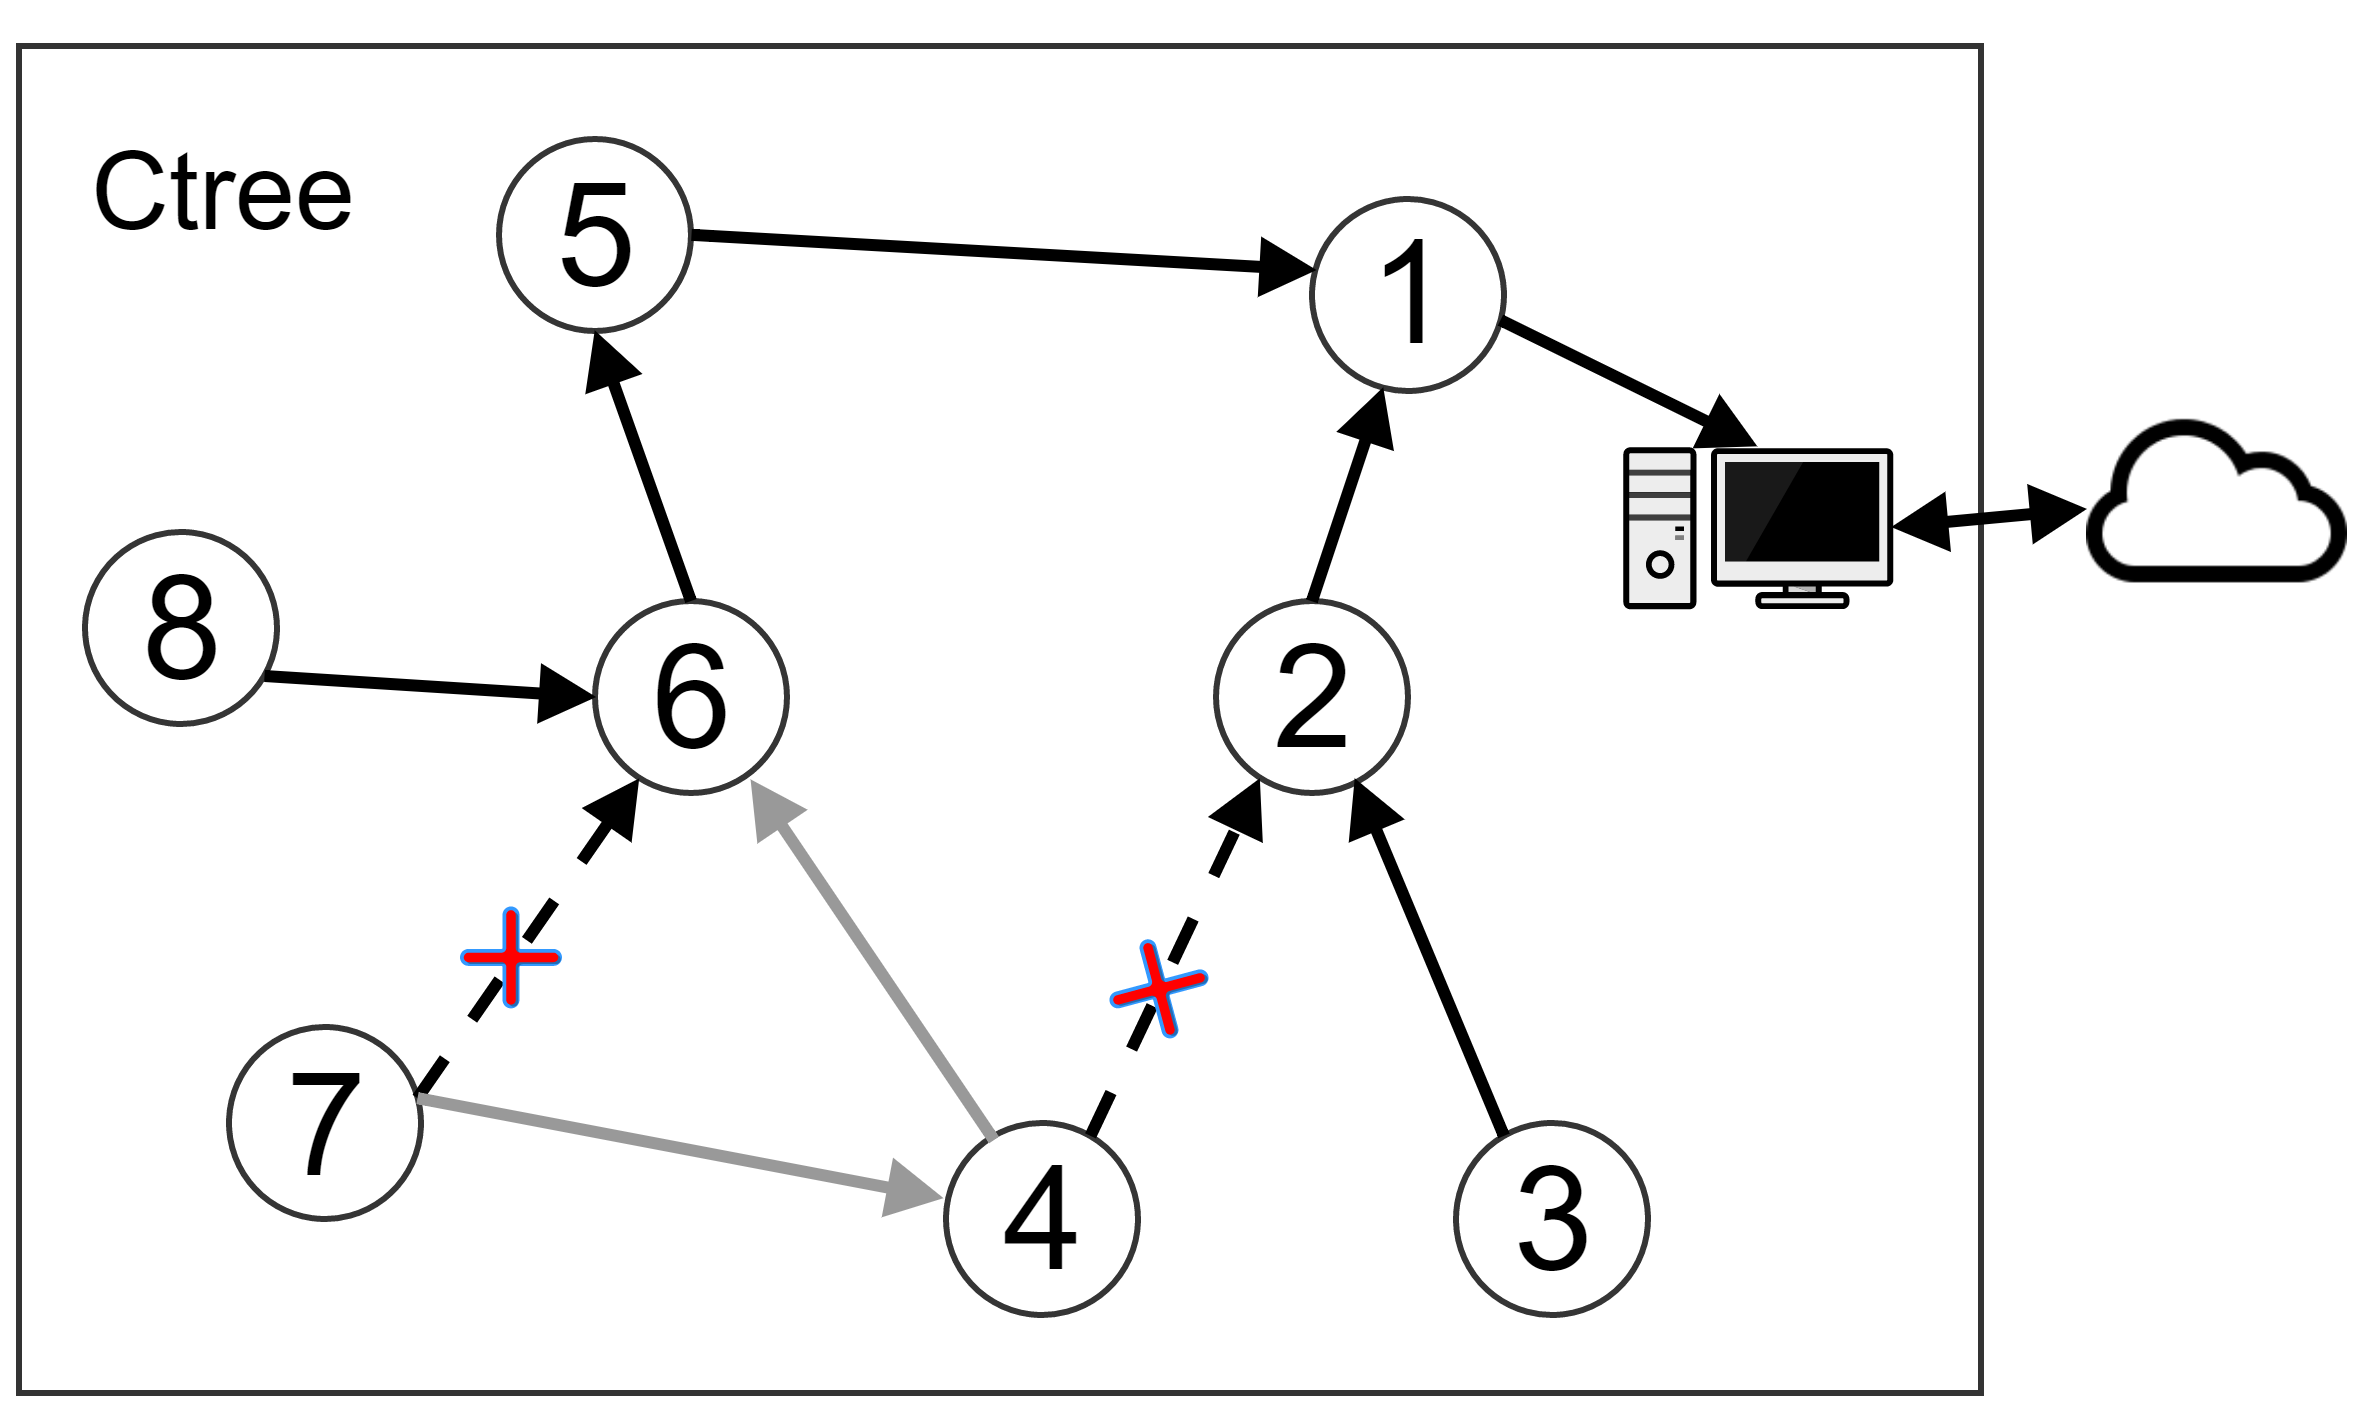
\includegraphics[width=.48\columnwidth]{Images/topologia3.png}
            \label{fig:t3}}
  \subfigure[]
  {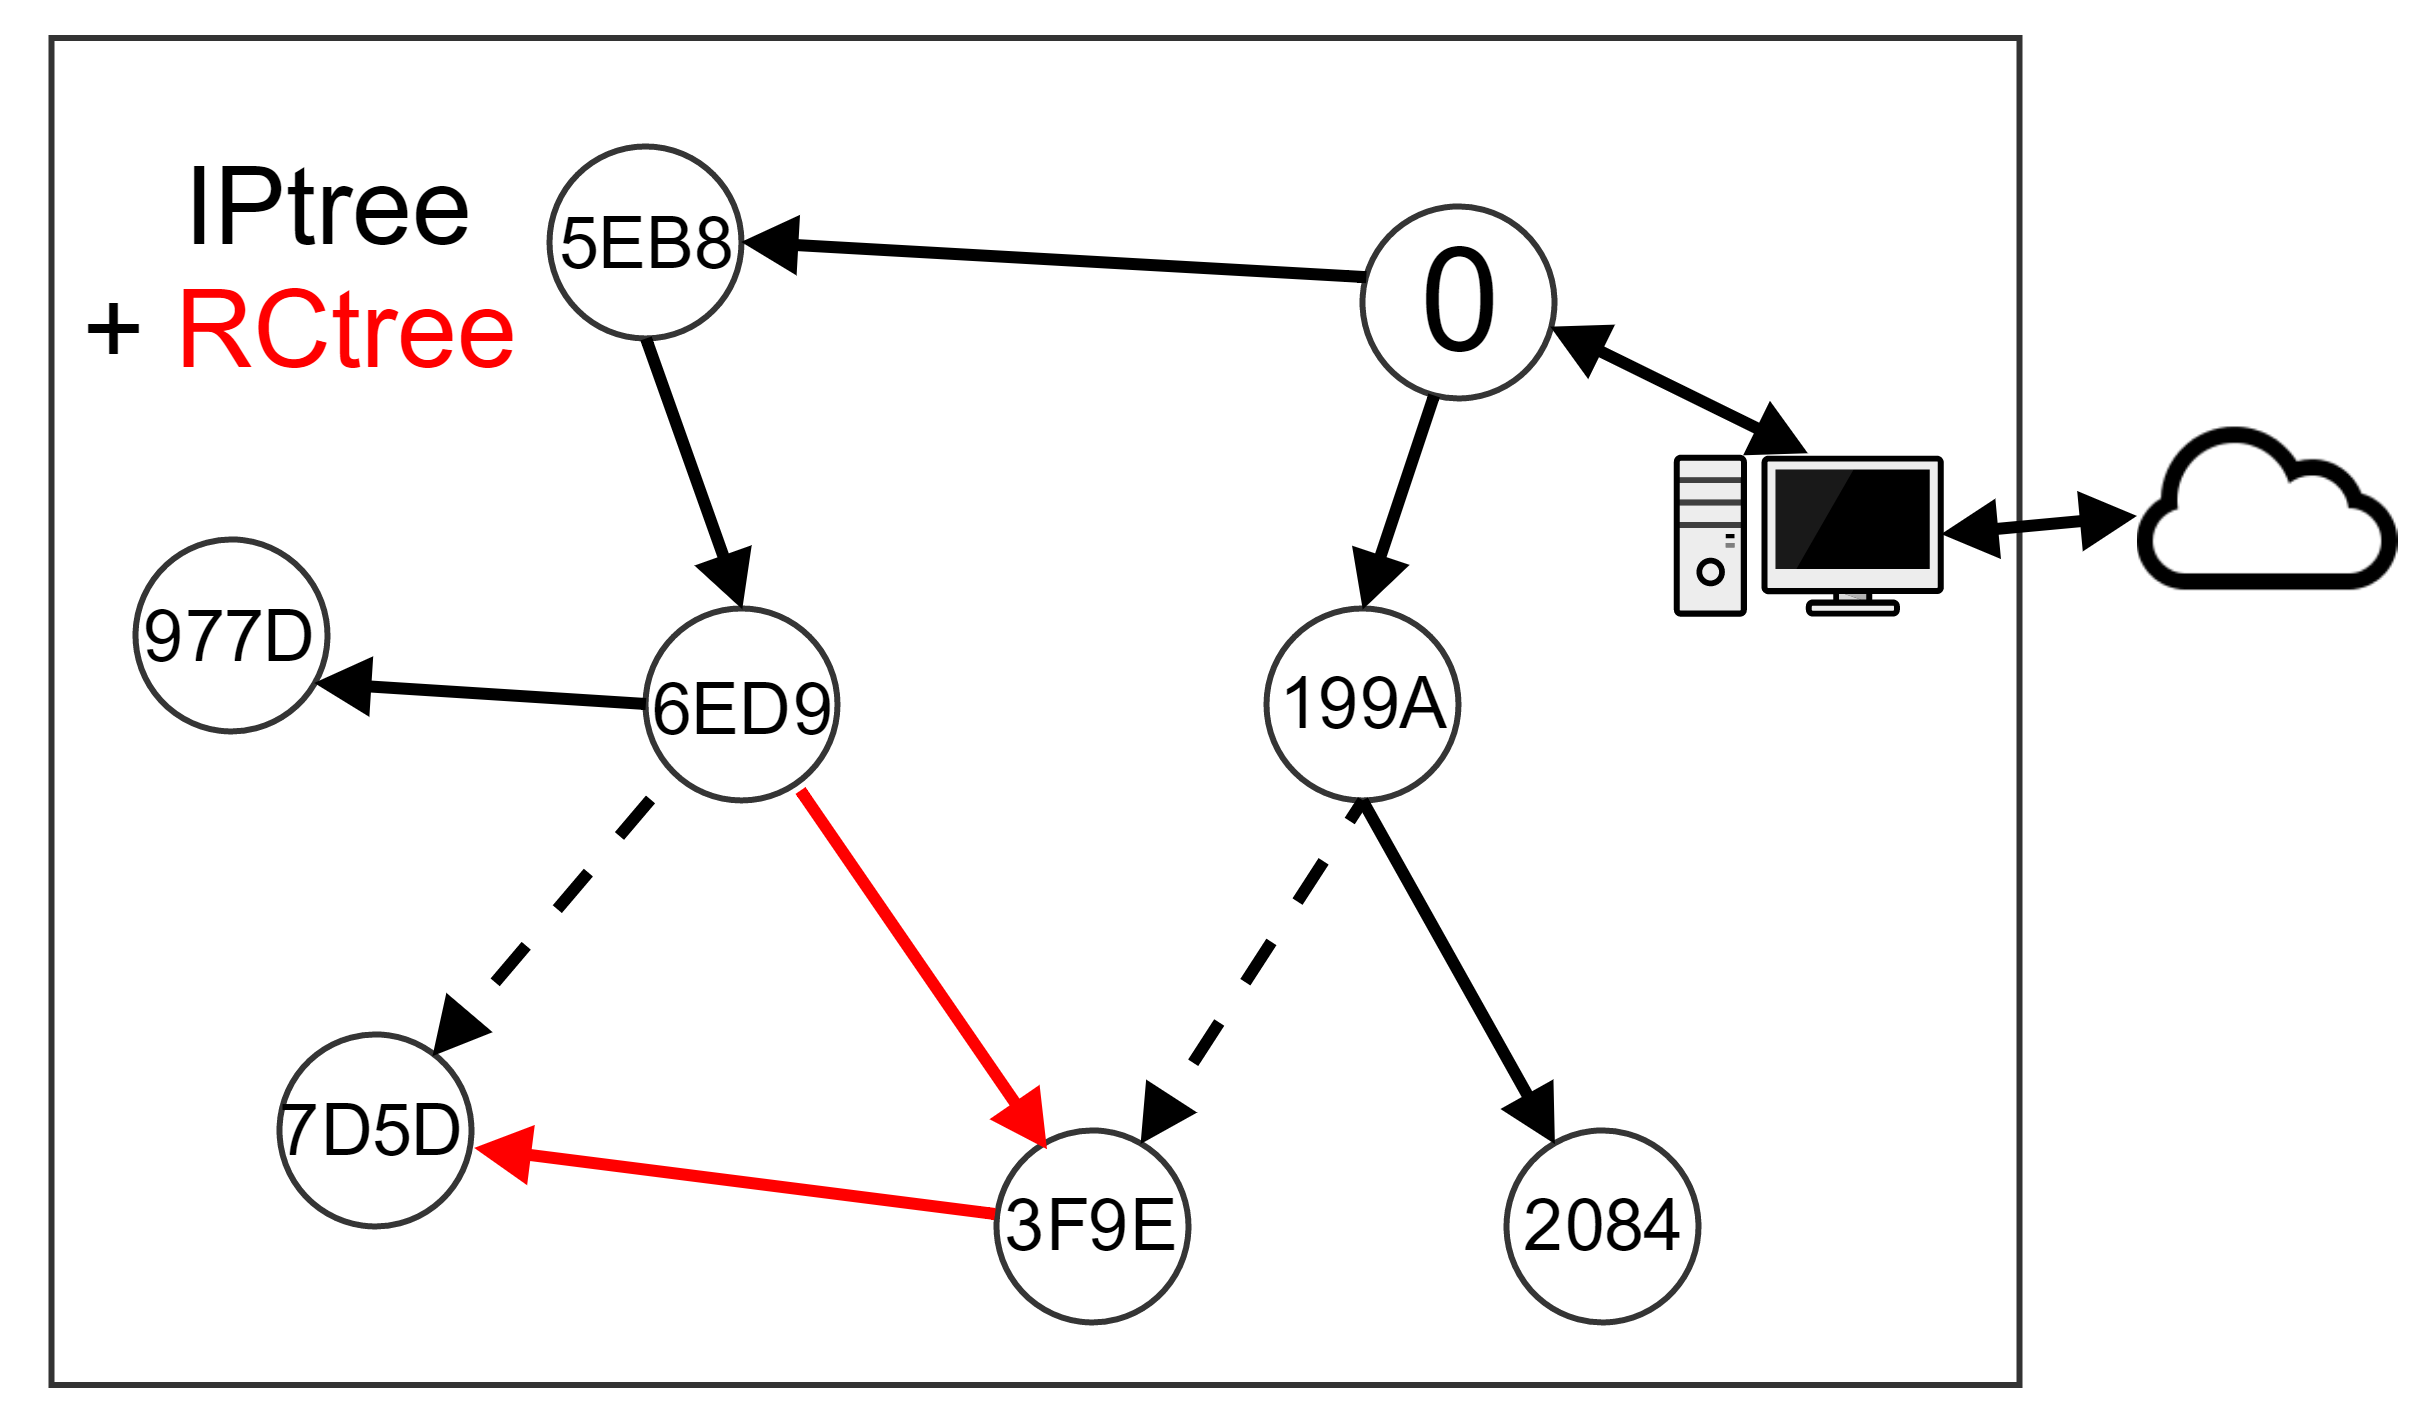
\includegraphics[width=.48\columnwidth]{Images/topologia4.png}
    \label{fig:t4}}
            \caption{RCtree example: before
            and after two links change in the collection tree.}\label{fig:layers}
\end{center}
\end{figure}

Each node $n_i$ maintains the following information:
\begin{itemize}
  \item $CTparent_i$: the ID of the current parent in the dynamic
  collection tree;
  \item $IParent_i$: the ID of the node that assigned $n_i$ its IPv6 range
initially $CTarent_i$ = $IParent_i$);
  \item $IPchildren_i$: the \textit{standard} (top-down) routing table, with
  address ranges of each one-hop descendent of $n_i$ in the IPtree;
  \item $RChildren_i$: the \textit{alternative} (top-down) routing table, with
  address ranges of one-hop descendants in the RCtree.
\end{itemize}

Note that, each node stores only one-hop
neighborhood information, so the memory footprint is $O(k)$, where $k$ is the
number of a node's children at any given moment in time, which is optimal,
considering that any (optimal) top-down routing mechanism would need at
least one routing entry for every (current) child in the tree topology to reach
all destinations.

The routing engine (see Figure~\ref{fig:architecture}) is responsible for
creating and maintaining the IPtree and RCtree routing tables. IPtree is created
during the network initialization phase, while RCtree is updated dynamically to
reflect changes in the network's link qualities. Whenever a node $n_i$ has its
$CTparent_i$ updated, and the current parent is different from its
$IParent_i$ ($IParent_i \neq CTparent_i$), $n_i$ starts sending periodic beacons
to its new parent, with regular intervals (in our experiments, we set the beacon
interval to $\delta/8$, where $\delta$ is the maximum interval of the
Trickle timer used in CTP).
Upon receiving a beacon (from a new child in the collection tree), a node
($n_j = CTparent_i$) creates and keeps an entry in its alternative
routing table $RChildren_j$ with the IPv6 address range of the subtree of $n_i$. As soon as $n_i$
stops using $n_j$ as the preferred parent, it stops sending beacons to $n_j$.
If no beacon is received from $n_i$ after $2\times\delta$ ms, its (alternative)
routing entry is deleted. Therefore, links in RCtree are temporary and are deleted when not present in neither the
collection nor the IP trees.

\subsection{Data plane: any-to-any routing}

The forwarding engine (see Figure~\ref{fig:architecture}) is responsible for
application packet forwarding. Any-to-any routing is performed by combining
  bottom-up forwarding, until the least common ancestor of sender and
  receiver, and then top-down forwarding until the destination. Upon receiving
  an application layer packet, each node $n_i$ verifies whether the destination IPv6 address falls within some range
$j \in IPchildren_i$: if yes then the packet is forwarded
(downwards) to node $n_j$, otherwise, the packet is forwarded
(upwards) to $CTparent_i$. Note that, since each node has an IPv6
address, in contrast to collection protocols, such as CTP and RPL,
in Matrix, every node can act as a destination of messages
originated inside and outside of the 6LoWPAN.

Each forwarded packet requests an acknowledgment from the next hop and can be
retransmitted up to 30 times (similarly to what is done in CTP
\cite{Fonseca:2009}). If thereafter no acknowledgment
is received, then the node performs a \textit{local broadcast}, looking for an
alternative next hop in the RCtree table of a (one-hop) neighbor. The
\textit{alternative routing} process is described in detail below.

\subsection{Fault tolerance and network dynamics}

So why is Matrix robust to network dynamics? Note that, since
routing is based on the hierarchical address allocation, if a node
with the routing entries necessary to locate the next subtree
becomes unreachable for longer than approximately one second
(failures that last less than 1s are effectively dealt with by
retransmission mechanisms available in standard link layer
protocols), messages with destinations in that subtree are dropped.

When a node or link fails or changes in Ctree, RCtree reflects this
change, and packets are forwarded from IPtree to RCtree via a local
broadcast. The node that receives a local-broadcast checks in its
RCtree whether it knows the subtree of the destination IPv6 address:
if yes then is forwards the packet to the right subtree and the
packet continues its path in the IPtree until the final destination.

\begin{figure}[!h]
\begin{center}
  \subfigure[]
  {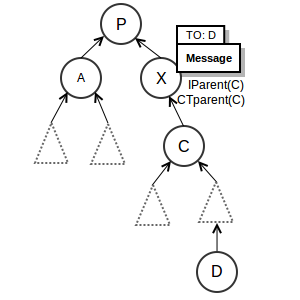
\includegraphics[width=.48\columnwidth]{Images/lb1.png}
            \label{fig:lb1}}
  \subfigure[]
  {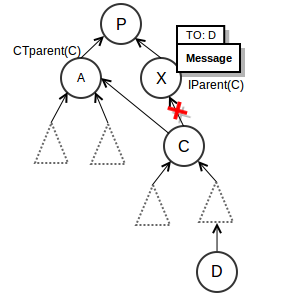
\includegraphics[width=.48\columnwidth]{Images/lb2.png}
                        \label{fig:lb2}}
                            \subfigure[]
  {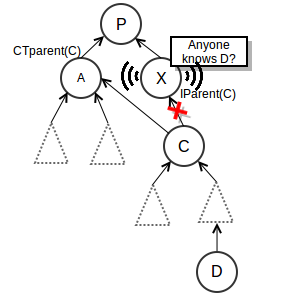
\includegraphics[width=.48\columnwidth]{Images/lb3.png}
            \label{fig:lb3}}
  \subfigure[]
  {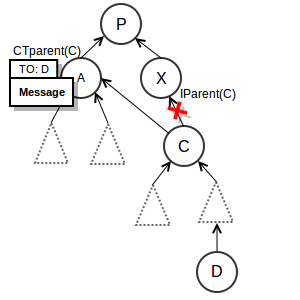
\includegraphics[width=.48\columnwidth]{Images/lb4.png}
    \label{fig:lb4}}
            \caption{Alternative top-down routing.}\label{fig:localbroadcast}
\end{center}
\end{figure}


Consider the following scenario: node X receives a packet with destination IPv6
address D (see Figure \ref{fig:lb1}). After consulting its standard routing
table $IP-children_X$, X forwards the packet to C. However, the link X
$\Rightarrow$ C fails, for some reason, and C does not reply with an
acknowledgment.
Then, X makes a constant number (e.g., 30 times in CTP) of retransmission
attempts. Meanwhile, since node C also lost its connection to X, it decides to
change its parent in the collection tree to node A (see Figure \ref{fig:lb2}).
Having changed its parent, C starts sending beacons to A, which creates an entry
in its alternative routing table $RC-children_A$ for the subtree rooted at C, and
keeps it as long as it receives periodic beacons from C (which will be done as long as $CTparent_C$ = A).

Having received no ack from C, X activates the \textit{local
broadcast} mode: it sets the message's type to ``LB'' and broadcasts
it to all its one-hop neighbors (see Figure \ref{fig:lb3}). Upon
receiving the local broadcast, node A consults its alternative
routing table and finds out that the destination address D falls
within the IPv6 address range C. It then forwards the packet to C,
from where the packets follows along its standard route in the
subtree of C (see Figure \ref{fig:lb4}).

Note that this
mechanism does not guarantee that the message will be delivered. If no one-hop
neighbor of X had the address range of C in its alternative routing table, then
the packet would be lost. Nevertheless, we argue that the probability that the
message will be forwarded to the appropriate subtree is high.

\subsection{Alternative routing: geometric rationale}
The success of the local broadcast mechanism lies in the ability to forward
messages top down along the IPtree, in spite of one or more link or node
failures on the way.
Matrix is designed to handle (non-adjacent) link or node failures and relies on
a single local broadcast and temporary reverse collection links (RCtree).

Consider once again the scenario illustrated in Figure \ref{fig:localbroadcast}.
When a node X is unable to forward a packet to the next hop, it activates the
local broadcast mechanism, and it becomes essential that one of X's one-hop
neighbors (in this case A) has replaced X as a parent of C in
the collection tree. Therefore, given that the new parent of C is A, it becomes
essential that X and A are neighbors. We argue that it is unlikely that this is not the case.

\begin{figure}[!ht]
    \centering
    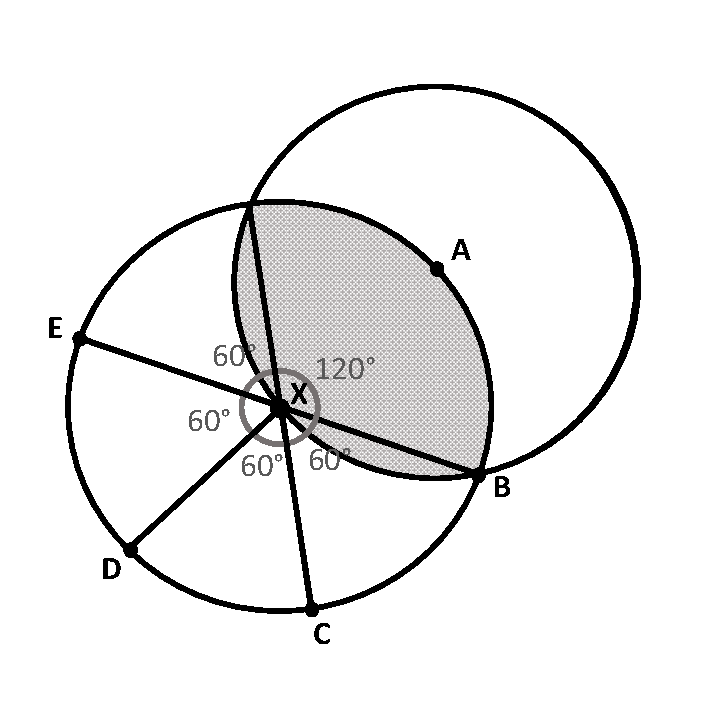
\includegraphics[width=.6\linewidth]{./Images/localbroad.pdf}
\caption{UDG model: the number of independent neighbors of X is at most 5.}
    \label{fig:udgIndN}
\end{figure}

Our argument is of geometric nature. Since the considered 6LoWPAN is
wireless, we show our argument in a unit disk graph (UDG) model
\cite{Clark:1991}. We use the fact that the number of independent neighbors of
any node in a UDG is bounded by a small constant, namely 5. The proof of this
fact is sketched in Figure \ref{fig:udgIndN}: consider a node X and its neighbor
A. Any node located inside the gray region is a neighbor of both X and A, so any
neighbor of X that is independent of (not adjacent to) A has to be outside the
gray area and inside the circle around X. Let's call this neighbor B. The next
independent neighbor of X has to be located outside the 60 degree sector that
starts at B, and so on. This procedure can be repeated no more than 5 times,
before the 360 degrees around X are covered.

Given that the maximum number of neighbors that do not know each
other is very small, for any possible node distribution and density
around X, the probability that two neighbors of X are independent is
low. In Figure \ref{fig:lb3}, since both X and A are neighbors of C,
the probability that they are themselves neighbors is high. Similar
arguments can be used to back the effectiveness of the local
broadcast mechanism when dealing with different non-adjacent link
and node failures.

Note that this reasoning is only valid in an open space without obstacles and,
even then, does not guarantee that the message will be delivered. Nevertheless,
our experiments show that this intuition is in fact correct, and Matrix has a
95\%--99\% message delivery success in scenarios with node failures of
increasing frequency and duration.
